\chapter{Otras funciones especiales}
\section{Funciones de Laguerre}
\subsubsection{Gr'aficos}
\begin{figure}[!h]
\centerline{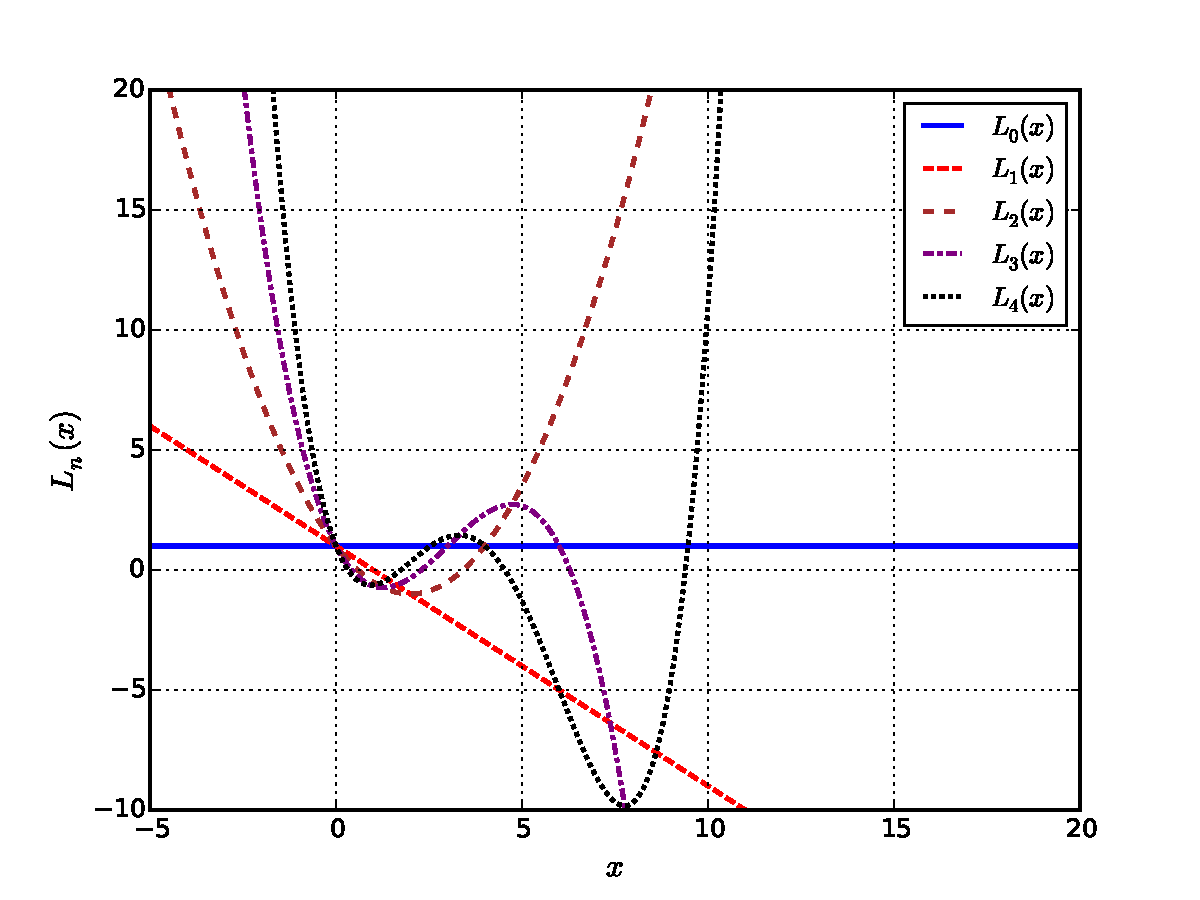
\includegraphics[height=7cm,angle=0]{figs/fig-Laguerre.pdf}}
\caption{Funciones de Laguerre}
\end{figure}

\subsubsection{Ecuaci'on diferencial}

\begin{equation}
x\frac{d^{2}y}{dx^{2}}+(1-x)\frac{dy}{dx}+ny=0
\end{equation}

\subsubsection{Ecuaci'on diferencial (forma de Sturm-Liouville)}

\begin{equation}
\frac{d}{dx}\left[\left(xe^{-x} \right)\frac{dy}{dx}\right]+ne^{-x}y=0
\end{equation}

\subsubsection{F'ormula de Rodrigues}

\begin{equation}
L_{n}(x)=\frac{e^{x}}{n!}\frac{d^{n}}{dx^{n}}(x^{n}e^{-x})
\end{equation}

\subsubsection{Funci'on generadora}

\begin{equation}
\frac{e^{-\frac{xt}{1-t}}}{(1-t)}=\sum_{n=0}^{\infty}\frac{L_{n}(x)}{n!}t^{n}
\end{equation}

\subsubsection{Relaciones de Recurrencia}

\begin{equation}
(n+1)L_{n+1}(x)=(2n+1-x)L_{n}(x)-n^{2}L_{n-1}(x)
\end{equation}

\subsubsection{Ortogonalidad}

\begin{equation}
\int_{0}^{\infty}L_{m}(x)L_{n}(x)e^{-x}\,dx=\delta_{mn}
\end{equation}

\newpage
\section{Funciones de Laguerre asociadas}

\subsubsection{Ecuaci'on diferencial}

\begin{equation}
x\frac{d^{2}y}{dx^{2}}+(k+1-x)\frac{dy}{dx}+ny=0
\end{equation}

\subsubsection{Ecuaci'on diferencial (forma de Sturm-Liouville)}

\begin{equation}
\frac{d}{dx}\left[\left(x^{k+1}e^{-x} \right)\frac{dy}{dx}\right]+ne^{-x}x^{k}y=0
\end{equation}

\subsubsection{F'ormula de Rodrigues}

\begin{equation}
L_{n}^{k}(x)=\frac{e^{x}x^{-k}}{n!}\frac{d^{n}}{dx^{n}}(x^{n+k}e^{-x})
\end{equation}

\subsubsection{Funci'on generadora}

\begin{equation}
(-1)^{k}\, t^{k} \frac{e^{-\frac{xt}{1-t}}}{(1-t)^{k+1}}=\sum_{n=0}^{\infty}\frac{L^{k}_{n}(x)}{n!}t^{n}
\end{equation}

\subsubsection{Relaciones de Recurrencia}

\begin{equation}
\frac{n-k+1}{n+1} L_{n+1}^{k}(x) + \Big(x+m-2n-1\Big) L_n^m(x) + n^2 L^m_{n-1}(x) = 0
\end{equation}


\subsubsection{Ortogonalidad}

\begin{equation}
\int_{0}^{\infty}L^k_{m}(x)L^k_{n}(x)e^{-x}x^{k}\,dx=\frac{\Gamma(n+k+1)!}{n!}\delta_{mn}
\end{equation}

\subsubsection{Aplicaci'on en F'isica}
\begin{itemize}
\item Soluci'on radial de ecuaci'on de Schr\"odinger en potencial de Coulomb ('atomo hidrogenoide).
\end{itemize}


\newpage
\section{Funciones de Hermite}

\subsubsection{Gr'aficos}
\begin{figure}[!h]
\centerline{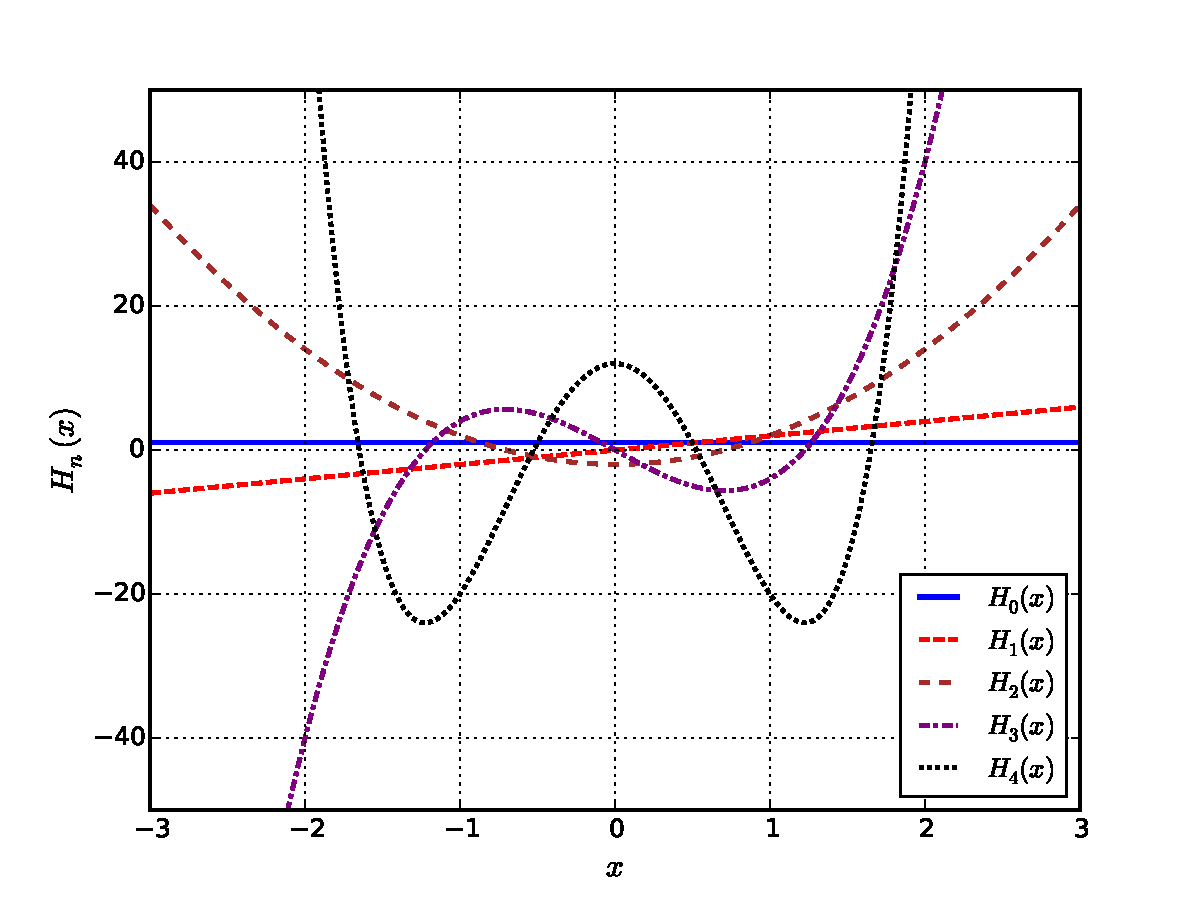
\psfig{file=figs/fig-Hermite.pdf,height=7cm,angle=0}}
\caption{Funciones de Hermite}
\end{figure}

\subsubsection{Ecuaci'on diferencial}

\begin{equation}
\frac{d^{2}y}{dx^{2}}-2x\frac{dy}{dx}+2ny=0
\end{equation}

\subsubsection{Ecuaci'on diferencial (forma de Sturm-Liouville)}

\begin{equation}
\frac{d}{dx}\left[\left( e^{-x^{2}}\right)\frac{dy}{dx}\right]+2ne^{-x^{2}}y=0
\end{equation}

\subsubsection{F'ormula de Rodrigues}

\begin{equation}
H_{n}(x)=(-1)^{n}e^{x^{2}}\frac{d^{n}}{dx^{n}}e^{-x^{2}}
\end{equation}

\subsubsection{Funci'on generadora}

\begin{equation}
e^{2tx-t^{2}}=\sum_{n=0}^{\infty}\frac{H_{n}(x)}{n!}t^{n}
\end{equation}

\subsubsection{Relaciones de Recurrencia}

\begin{equation}
H_{n+1}(x)=2xH_{n}(x)-2nH_{n-1}(x)
\end{equation}

\subsubsection{Ortogonalidad}
\begin{equation}
\int_{-\infty}^{\infty}H_{m}(x)H_{n}(x)e^{-x^{2}}\,dx=2^{n}n!\sqrt{\pi}\delta_{mn}
\end{equation}

\subsubsection{Aplicaci'on en F'isica}
\begin{itemize}
\item Oscilador arm'onico cu'antico
\end{itemize}

\newpage
\section{Polinomios de Chebyshev}
\subsubsection{Gr'aficos}
\begin{figure}[!h]
\centerline{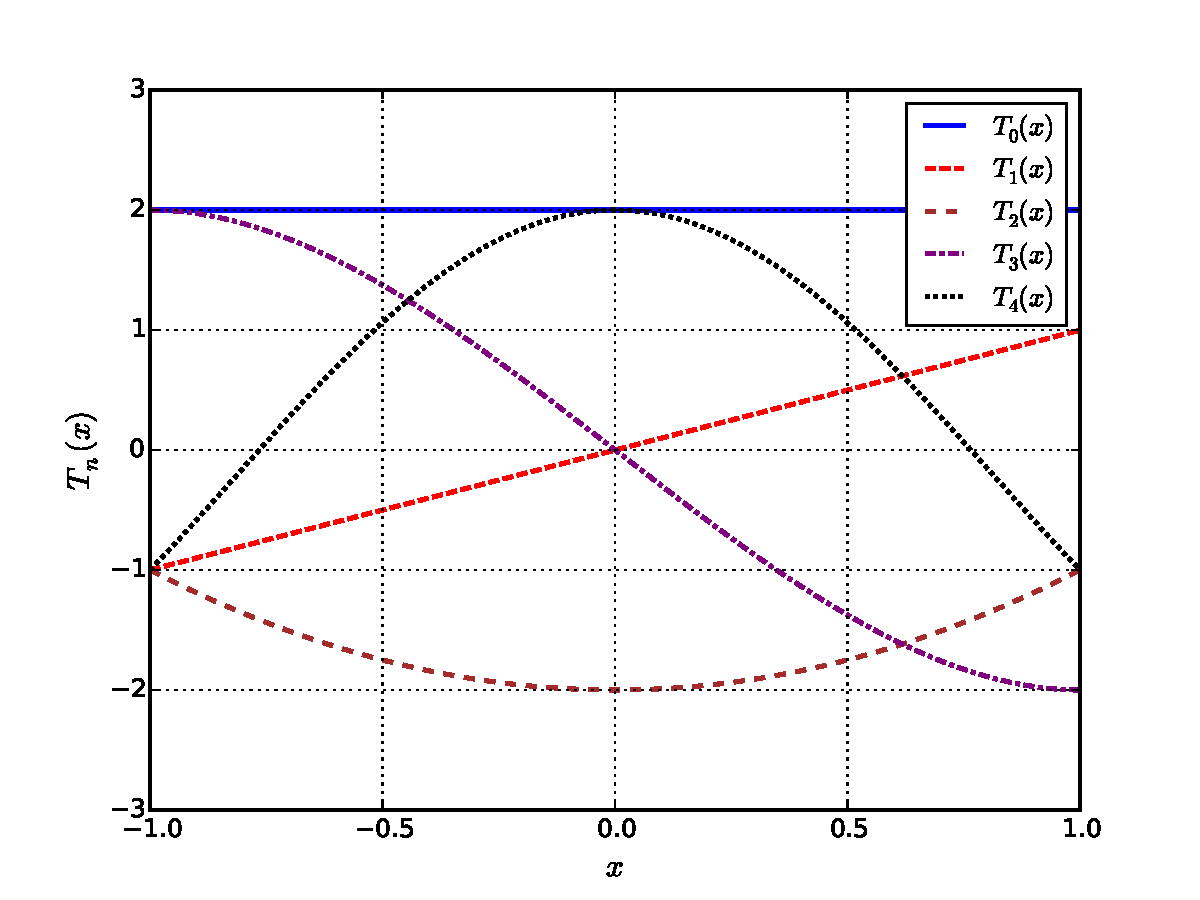
\psfig{file=figs/fig-Chebyshev.pdf,height=7cm,angle=0}}
\caption{Polinomios de Chebyshev}
\end{figure}
\url{http://en.wikipedia.org/wiki/File:Chebyshev_Polynomials_of_the_1st_Kind_(n\%3D0-5,_x\%3D(-1,1)).svg}


\subsubsection{Ecuaci'on diferencial}

\begin{equation}
(1-x^{2})\frac{d^{2}y}{dx^{2}}-x\frac{dy}{dx}+n^{2}y=0
\end{equation}

\subsubsection{Ecuaci'on diferencial (forma de Sturm-Liouville)}

\begin{equation}
\frac{d}{dx}\left[\left(\sqrt{1-x^{2}} \right)\frac{dy}{dx}\right]+\frac{n^{2}}{\sqrt{1-x^{2}}}y=0
\end{equation}

\subsubsection{F'ormula de Rodrigues}

\begin{equation}
T_{n}(x)=\frac{(-1)^{n}\sqrt{1-x^{2}}}{(2n-1)(2n-3)\cdots 1} \frac{d^{n}}{dx^{n}}(1-x^{2})^{n-\frac{1}{2}}
\end{equation}

\subsubsection{Funci'on generadora}

\begin{equation}
\frac{1-tx}{1-2tx+t^{2}}=\sum_{n=0}^{\infty}T_{n}(x)t^{n}
\end{equation}

\subsubsection{Relaciones de Recurrencia}

\begin{equation}
T_{n+1}(x)=2xT_{n}(x)-T_{n-1}(x)
\end{equation}

\subsubsection{Ortogonalidad}

\begin{equation}
\int_{-1}^{1}\frac{T_{m}(x)T_{n}(x)}{\sqrt{1-x^{2}}}\,dx= \left\{\begin{array}{ll}\pi & m=n=0\\ \frac{\pi}{2}\delta_{mn} & m=n=N \in \mathbb{N} \end{array}\right.
\end{equation}

\subsubsection{Aplicaci'on en F'isica}
\begin{itemize}
\item ??
\end{itemize}